\subparagraph{Задание 4.12}

\textbf{Условие}: Вывести содержимое выходного буфера в окне Watches. 

\textbf{Решение}:

В Turbo Debugger захожу в меню клавишей \textbf{F10}. Два раза перемещаюсь \textbf{вправо}. Выбираю вкладку \textbf{View}. \textbf{Enter}. Два раза перемещаюсь \textbf{вниз}. Выбираю вкладку \textbf{Watches}. \textbf{Enter}.
Рисунок~\ref{fig:task_4_12__1} (стр.~\pageref{fig:task_4_12__1}).
Ввожу c клавиатуры \textbf{cx}.
Рисунок~\ref{fig:task_4_12__2} (стр.~\pageref{fig:task_4_12__2}).
Видим снизу в Watches коробке \textbf{cx word 38136 (94F8h)}.
Рисунок~\ref{fig:task_4_12__3} (стр.~\pageref{fig:task_4_12__3}).

\begin{figure}[!htp]
    \centering
    \begin{minipage}{0.32\textwidth}
        \centering
        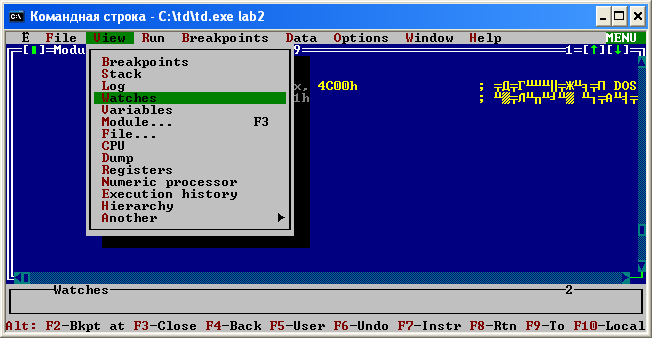
\includegraphics[width=.99\linewidth]
            {../_INCLUDES/task-4-12/1.png}
        \caption{1) \textbf{Watches}}
        \label{fig:task_4_12__1}
    \end{minipage}
    \begin {minipage}{0.32\textwidth}
        \centering
        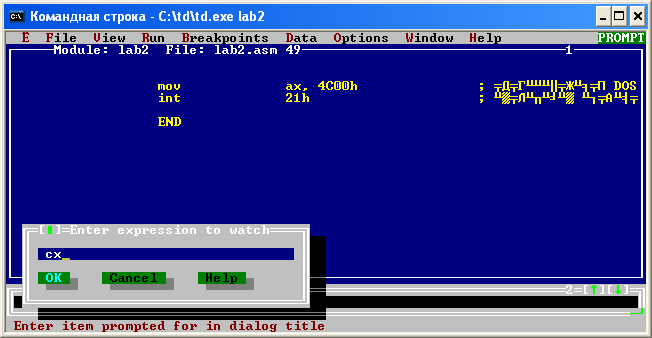
\includegraphics[width=.99\linewidth]
            {../_INCLUDES/task-4-12/2.png}
        \caption{2) Вводим \textbf{cx}}
        \label{fig:task_4_12__2}
    \end{minipage}
    \begin {minipage}{0.32\textwidth}
        \centering
        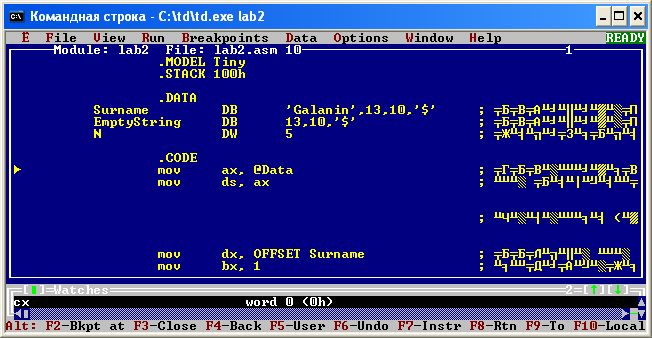
\includegraphics[width=.99\linewidth]
            {../_INCLUDES/task-4-12/3.png}
        \caption{3) Результат}
        \label{fig:task_4_12__3}
    \end{minipage}
\end{figure}
